\begin{frame}{Deciding functions}
\begin{itemize}
\item A very important, recurring problem is \emph{deciding} a finite \alert{function}.
\item Given 
\begin{itemize}
\item[-] Domain \texttt{DOM}
\item[-] Codomain \texttt{COD}
\end{itemize} 
\item Find a function $f : \mathtt{DOM} \to \mathtt{COD}$ 
\item Satisfying some criteria (e.g. \emph{injectivity})
\end{itemize}
\vspace*{1ex}
\pause 
Examples:
\begin{itemize}
\item Task allocation (maps tasks to workers, exactly one worker per task)
\item Exam schedules (map students to appointments, certainly different appointments)
\end{itemize}
\end{frame}

\begin{frame}{Task allocation in practice}

\vspace*{1cm}

\begin{itemize}
\item Task allocation problem

\begin{itemize}
\item [-] $n$ robots 
\item [-] $m$ tasks
\item [-] Assign each robot a \emph{different} task and maximize the profit
\end{itemize}
\item Example:
\begin{itemize}
\item[-] $n = 4$, $m = 5$
\end{itemize}
\end{itemize}
\centering
\begin{tabular}{|c|c|c|c|c|c|}
\hline 
 & t1 & t2 & t3 & t4 & t5 \\ 
\hline 
r1 & 7 & 1 & 3 & 4 & 6 \\ 
\hline 
r2 & 8 & 2 & 5 & 1 & 4 \\ 
\hline 
r3 & 4 & 3 & 7 & 2 & 5 \\ 
\hline 
r4 & 3 & 1 & 6 & 3 & 6 \\ 
\hline 
\end{tabular} 

\begin{textblock*}{5.5cm}[1,1](\textwidth-1cm,\textheight-5.33cm)
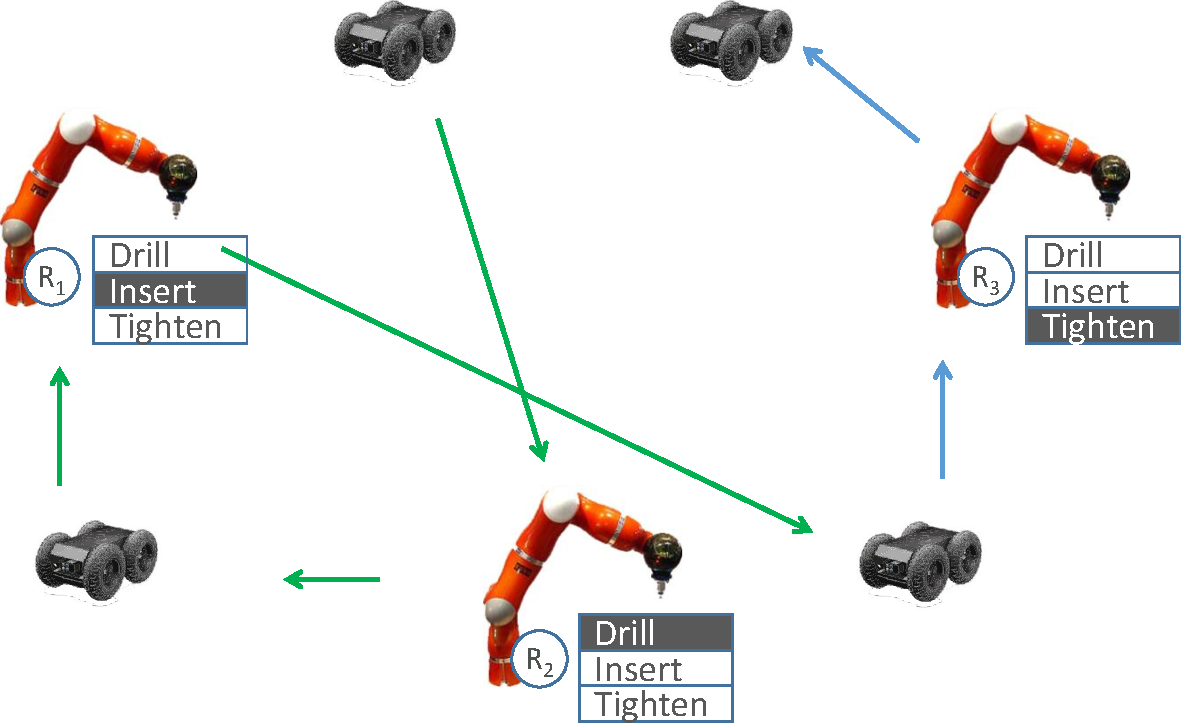
\includegraphics[width=.7\textwidth]{img/produktionszelle.pdf}
\end{textblock*}

\end{frame}


\begin{frame}[fragile]{Task allocation: Model}
\begin{lstlisting}
% problem data 
int: n; set of int: ROBOTS = 1..n;
int: m; set of int: TASKS = 1..m;
array[ROBOTS,TASKS] of int: profit;

% decisions
array[ROBOTS] of var TASKS: allocation;

% goal
solve maximize sum(r in ROBOTS) (profit[r, allocation[r]] );

% have robots work on different tasks
constraint forall(r1 in ROBOTS, r2 in ROBOTS where r1 < r2) 
  ( allocation[r1] != allocation[r2] );
\end{lstlisting}
\end{frame}

\begin{frame}[fragile]{Judgement}
\begin{lstlisting}
constraint forall(r1 in ROBOTS, r2 in ROBOTS where r1 < r2) 
  ( allocation[r1] != allocation[r2] );
\end{lstlisting}
\begin{itemize}
\item In principle, \emph{fine}, but \ldots
\begin{itemize}
\item[-] Not very concise -- can be messed up
\item[-] $O(n^2)$ individual constraints between two variables
\end{itemize}
\pause 

\vspace*{1ex}

\item But in fact, this substructure is so common that it deserves a \emph{name}
\begin{itemize}
\item[-] \texttt{alldifferent}
\end{itemize}
\end{itemize}
\begin{lstlisting}
constraint alldifferent(allocation);
\end{lstlisting}
\begin{itemize}
\item $\mathrm{alldifferent}([x_1, \ldots, x_n]$ is true if and only if all variables $x_1$ to $x_n$ take a different value
\item e.g. $\mathrm{alldifferent}([2,3,5])$ holds but $\mathrm{alldifferent}([2,2,3])$ does not.
\end{itemize}
\end{frame}

\begin{frame}[fragile]{Task allocation: Improved Model}
\begin{lstlisting}
% problem data 
int: n; set of int: ROBOTS = 1..n;
int: m; set of int: TASKS = 1..m;
array[ROBOTS,TASKS] of int: profit;

% decisions
array[ROBOTS] of var TASKS: allocation;

% goal
solve maximize sum(r in ROBOTS) (profit[r, allocation[r]] );

include "alldifferent.mzn"; % we have to import from the library
% have robots work on different tasks
constraint alldifferent(allocation);
\end{lstlisting}
\end{frame}

\begin{frame}[fragile]{AllDifferent -- Propagation}

\begin{lstlisting}
var {1,2,3}: x;       var {2,3}: y;      var {2,3}: z;
var {1,2,3,4,5}: t; var {3,4,5,6}: u;
constraint alldifferent([x,y,z,t,u]);
\end{lstlisting}
\vspace*{-15ex}
\begin{center}
\tikzset{onslide/.code args={<#1>#2}{%
  \only<#1>{\pgfkeysalso{#2}}
}}
\tikzstyle{highlight}=[isseorange,ultra thick]
\tikzstyle{impo}=[dashed]
\begin{tikzpicture}[every node/.style={
anchor=base,
text depth=.5ex,
text height=2ex,
minimum height=2ex,
align=center,
circle,
text width=1em}]
\matrix (magic) [nodes in empty cells, ampersand replacement=\&,row sep=0.3cm,column sep=0.5cm]
{
\node[draw, circle](x){$x$}; \& \node[draw, circle](y){$y$};  \& \node[draw, circle](z){$z$};  \& \node[draw, circle](t){$t$};  \& \node[draw, circle](u){$u$};  \\
 \& \\
\& \\
\& \\
\node[draw, circle](1){$1$};  \& \node[draw, circle](2){$2$};  \& \node[draw, circle](3){$3$};  \& \node[draw, circle](4){$4$};  \& \node[draw, circle](5){$5$};  \& \node[draw, circle](6){$6$};  \\
};

\draw[onslide={<2>{highlight}}] (x) -- (1);
\draw[onslide={<2>{impo}}] (x) -- (2);
\draw[onslide={<2>{impo}}] (x) -- (3);

\draw[onslide={<2>{highlight}}] (y) -- (3);
\draw[] (y) -- (2);

\draw[onslide={<2>{highlight}}] (z) -- (2);
\draw[] (z) -- (3);

\draw[onslide={<2>{highlight}}] (t) -- (5);
\draw[onslide={<2>{impo}}] (t) -- (1);
\draw[onslide={<2>{impo}}] (t) -- (2);
\draw[onslide={<2>{impo}}] (t) -- (3);
\draw[] (t) -- (4);
\draw[onslide={<2>{highlight}}] (u) -- (4);
\draw[onslide={<2>{impo}}] (u) -- (3);
\draw[] (u) -- (5);
\draw[] (u) -- (6);
\end{tikzpicture}
\end{center}
\vspace*{-15ex}
\begin{lstlisting}
var {1}: x;       var {2,3}: y;      var {2,3}: z;
var {4,5}: t;      var {4,5,6}: u;
constraint alldifferent([x,y,z,t,u]);
\end{lstlisting}
\end{frame}

\begin{frame}{Other Globals}
Assume an employee scheduling problem (rostering) 

(Shifts: 1 = morning, 2 = afternoon, 3 = night):

%\vspace*{2ex}
\begin{center}
\begin{tabular}{|c|c|c|c|c|c|}
\hline 
 & Monday & Tuesday & Wednesday & Thursday & Friday \\ 
\hline 
Nurse 1 & off & 1 & \alert<2->{2} & 3 & 2 \\ 
Nurse 2 & 1 & off & \alert<2->{1} & 1 & 1 \\ 
Nurse 3 & 1 & 2 & off & 1 & 2 \\ 
Nurse 4 & 2 & 2 & \alert<2->{2} & off & 3 \\ 
Nurse 5 & \alert<3->{3} & \alert<3->{3} & \alert<2->{2} & \alert<3->{3} & off \\ 
\hline 
\end{tabular} 
\end{center}
\pause 
\begin{itemize}
\item Consider work regulations
\begin{itemize} \pause 
\item At least one nurse has to be assigned to every shift per day \pause 
\item Each nurse may at most work two night shifts
\item Each nurse needs to have one day off 
\end{itemize}
\end{itemize}

\begin{textblock*}{2.5cm}[1,1](\textwidth-2cm,\textheight-7.33cm)

\includegraphics[width=\textwidth]{img/nurse.jpg}
\end{textblock*}

\end{frame}

\begin{frame}[fragile]{Cardinality Constraint}

\begin{center}
\begin{tabular}{|c|c|c|c|c|c|}
\hline 
$\mathsf{worksShift}$ & Monday & Tuesday & Wednesday & Thursday & Friday \\ 
\hline 
Nurse 1 & off & 1 & 2 & 3 & 2 \\ 
Nurse 2 & 1 & off & 1 & 1 & 1 \\ 
%Nurse 3 & 1 & 2 & off & 1 & 2 \\ 
%Nurse 4 & 2 & 2 & 2 & off & 3 \\ 
%Nurse 5 & 3 & 3 & 2 & 3 & off \\ 
\hline 
\end{tabular} 
\end{center}%
\begin{itemize}
\item $\mathrm{cardinality}(X \mid v, l, u)$
\begin{itemize}
\item $X = \{x_1, \ldots, x_n\}$
\item $v = (v_1, \ldots, v_m)$
\item $l = (l_1, \ldots, l_m)$ contain \emph{lower} and 
$u = (u_1, \ldots, u_m)$ \emph{upper} bounds for values $v_i$ 
\end{itemize}

\vspace*{1ex} \pause

\item For instance, for each nurse $i$:
\begin{itemize}
\item[-] $\mathrm{cardinality}([ \mathsf{worksShift}[i, \cdot] ] \mid (0,1,2,3), (1,0,0,0), (5, 5, 5, 2))$
\end{itemize} 
\item In MiniZinc:
\end{itemize}
\begin{lstlisting}
constraint forall(i in NURSES) (
       global_cardinality_low_up([worksShift[i,d] | d in DAYS], 
                                 [0,1,2,3], [1,0,0,0], [1,5,5,2] ) );
\end{lstlisting}
\end{frame}